%% !TEX root = manual.tex

\section{Network Model}
\label{sec:tutorial:networkmodel}

Network models can be divided into several categories.  SST/macro supports analytic models, which estimate network delays via basic latency/bandwidth formulas, and packet models, which model step-by-step the transit of individuals through the interconnect.
A third class of models (flow models), was previously supported but are now discontinued due to the much better scalability of packet models.

\subsection{Analytic Models: MACRELS}
\label{subsec:tutorial:macrels}

The analytic models in SST/macro are colloqiually referred to as MACRELS (MTL for AnalytiC REally Lightweight Simulation).
An example file running a simple application can be found in the top-level examples folder.
The MTL (message transfer layer) moves entire network flows from point-to-point without packetizing them into smaller chunks.
Thus an entire 1 MB MPI message is transported as a single chunk of data.
The majority of MACRELS models are based on the LogP set of approximations:

\[
\Delta t = \alpha + \beta N
\]
where $\Delta t$ is the time delay, $\alpha$ is the minimum latency of the communication, $\beta$ is the inverse bandwidth (s/B), and N is the number of bytes.
In abstract machine models, these methods are selected as:

\begin{ViFile}
congestion_model = logP
\end{ViFile}
Details are shown for traffic moving from source to destination in Figure \ref{fig:macrelsOverview}.
Modeling occurs on entire flows, rather than individual packets. 

\begin{enumerate}
\item Flows queue waiting for NIC injection link to become available. Flow is forwarded to destination NIC based after computed delay. 
\item Flows queue waiting for NIC ejection link to become available. Flow finishes after ejection link becomes available.
\end{enumerate}

\begin{figure}
\centering
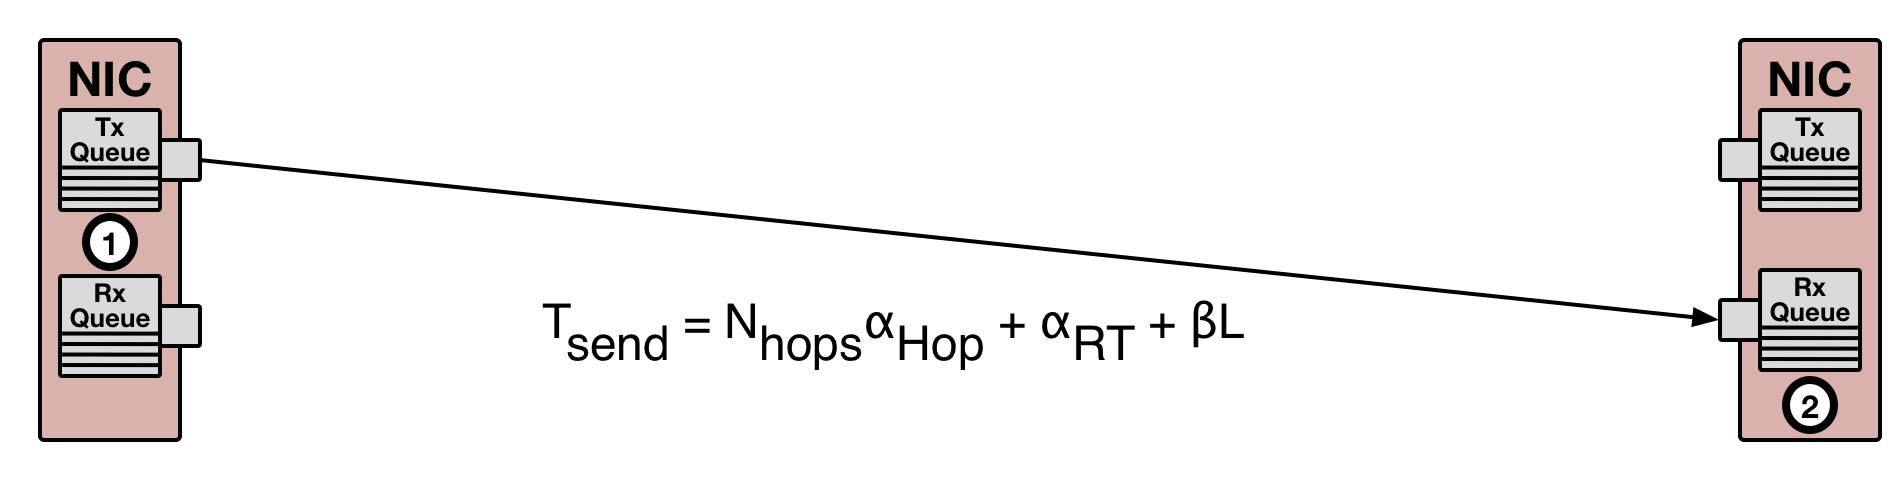
\includegraphics[width=0.9\textwidth]{figures/macrels.png}
\caption{MACRELS (Messages with AnalytiC REally Lightweight Simulation) skips congestion modeling and approximates send delays using a simple latency/bandwidth estimate, similar to the LogGOP model. Modeling occurs on entire flows, rather than individual packets. For details on numbered steps, see text.}
\label{fig:macrelsOverview}
\end{figure}


\subsection{Packet Models: PISCES}
\label{subsec:tutorial:pisces}

PISCES (Packet-flow Interconnect Simulation for Congestion at Extreme Scale) breaks network flows (MPI messages) into individual packets and models each packet individually.
An example file running a simple application can be found in the top-level examples folder.
In reality, packets are further subdivided into flits (flow-control units).
Flit-level detail would be way too computationally intense for large-scale simulation.
All routing decisions are made on packets as a while. 
Two flits in the same packet cannot take different paths through the network.
However, they may not travel together.

PISCES (Packet-flow Interconnect Simulation for Congestion at Extreme-Scale) models individual packets moving through the network. Flits (flow-control units) are approximately modeled using flow-like approximations. Packets can have partial occupancies in several different buffers, approximating wormhole routing. However, arbitration is modeled on whole packets, not individual flits (see Figure \ref{fig:piscesOverview})
\begin{enumerate}
\item A message (flow) is broken up into packets. Depending on available space in the Tx buffer, a limited number of packets may be able to queue up in the buffer. If credits are available in the Rx buffer for the link and the link is idle, the packet moves into the next Rx buffer after a computed delay.
\item The router selects a path for the packet and the packet requests to the crossbar to transmit to the corresponding output port. If credits are available for the Rx buffer, the crossbar may select the packet in arbitration and move it to the output buffer. After moving, the Rx buffer returns credits to the previous Tx buffer for that packet.
\item Step 1 is repeated for the next Rx buffer, waiting for credits and link availability.
\item Repeat Step 2
\item Repeat Step 3
\item Packet arrives in NIC Rx queue and queues waiting to inject into local memory. After injection, the Rx buffer returns credits to the corresponding Tx buffer.
\end{enumerate}

\begin{figure}[h!]
\centering
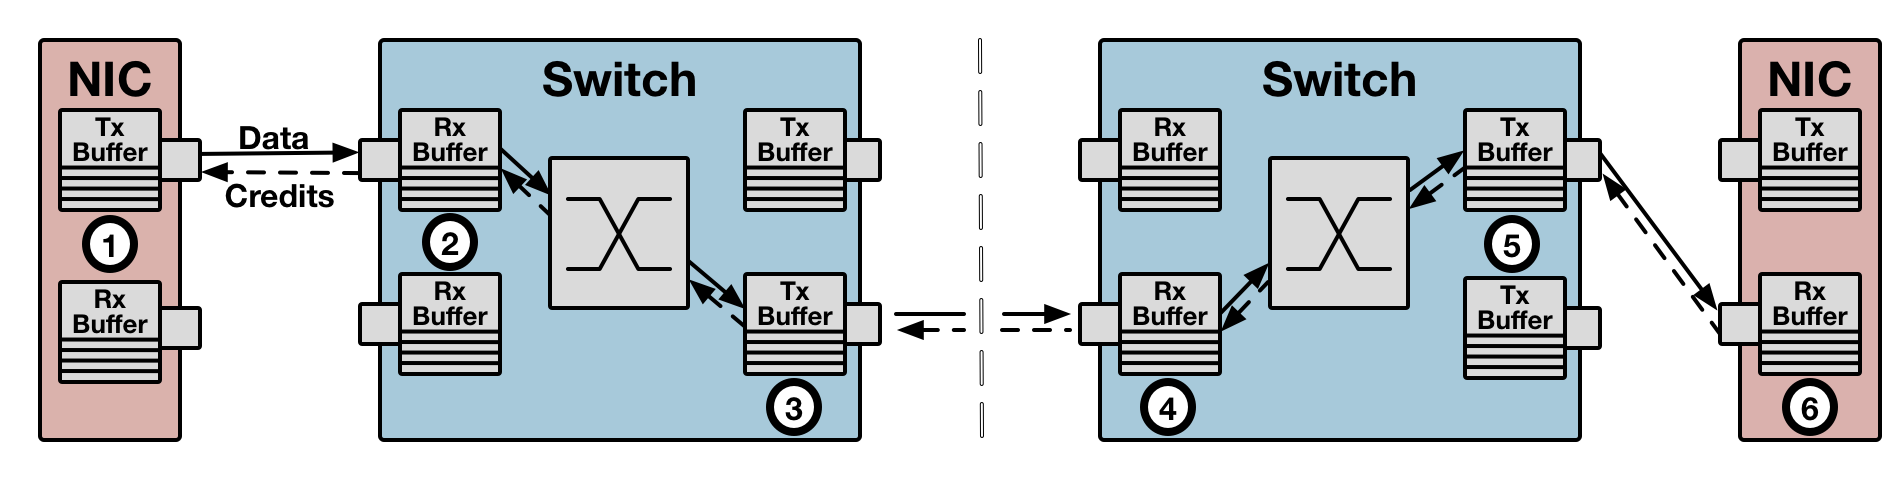
\includegraphics[width=0.9\textwidth]{figures/pisces_overview.png}
\caption[PISCES model]{PISCES (Packet-flow Interconnect Simulation for Congestion at Extreme-Scale) models individual packets moving through the network. Flits (flow-control units) are approximately modeled using flow-like approximations. For details on numbered steps, see text.}
\label{fig:piscesOverview}
\end{figure}


PISCES provides two mechanisms for treating flit-level flow control discussed next.

\subsubsection{PISCES simple model}
\label{subsubsec:tutorial:simplePisces}
In the simple model, each router uses a basic store-and-forward mechanism.
Flits are not allowed to ``separate'' and always travel as a single unit.
The entire packet has to be stored within a router before it can be forwarded to the next router.
The simple model affects the arbitrator that decided when and how to transmit flits.
To select a simple model:

\begin{ViFile}
arbitrator = simple
\end{ViFile}
The simple model is the least computationally expensive. 
However, for large packet sizes, it can produce erroneously high latencies.
To tune the packet size for abstract machine models, set:

\begin{ViFile}
switch.mtu = 1024B
node.nic.mtu = 1024B
\end{ViFile}
which sets the packet size to 1024B. 
For the simple model, packet sizes larger than 256-512B are not recommended.
Packet sizes on production supercomputers are often small (96-128B).
Small packet sizes with the simple model can be a good compromise for having more fine-grained routing but cheaper congestion modeling in the arbitrator.
More details are given in Figure \ref{fig:piscesOverview}.

\subsubsection{PISCES cut-through model}
\label{subsubsec:tutorial:cutThroughPisces}

\begin{figure}
\centering
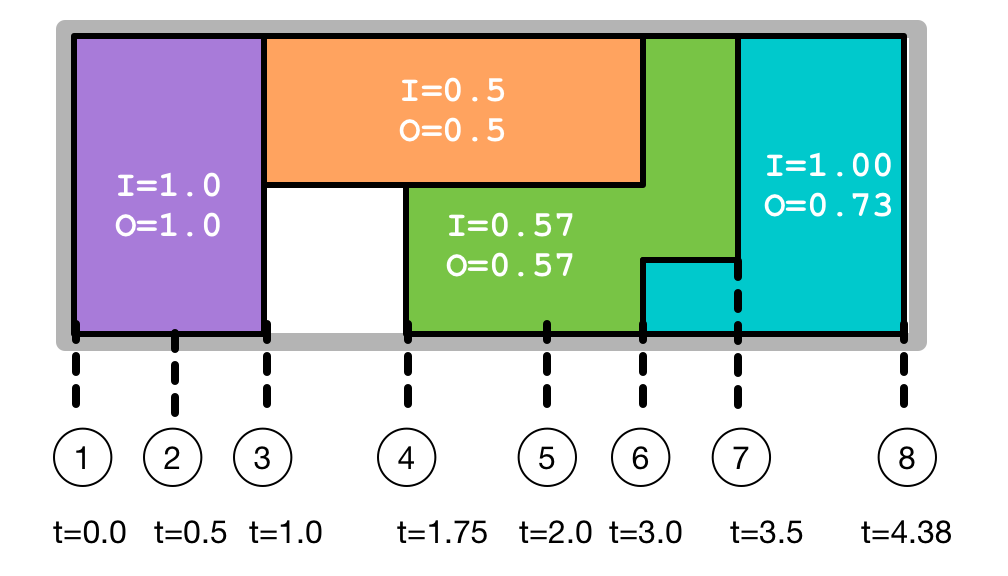
\includegraphics[width=0.6\textwidth]{figures/Pisces.png}
\caption{Timeline of four different packets passing through a PISCES cut-through bandwidth arbitrator. The incoming bandwidth (I) and outgoing bandwidth (O) are shown for each packet.  Time is the horizontal axis. Bandwidth consumed by a packet is shown by the vertical extent of each packet. The individual events are 1) First packet arrives 2) Second packet arrives with reduced bandwidth but no available bandwidth 3) First packet finishes. Second packet can begin sending. 4) Third packet arrives and begins sending with remaining bandwidth. 5) Fourth packet arrives, but no available bandwidth. 6) Second packet finishes. Third packet increases bandwidth. Fourth packet can begin sending. 7) Third packet finishes. Fourth packet increases bandwidth. 8) Fourth packet finishes.
Full details are given in the text.}
\label{fig:pisces}
\end{figure}

In the cut-through model, routing decisions still occur at the packet-level.
However, some attempt is made to account for pipelining of flits across different router stages.
Somewhat similar to the LogP models used above, latency/bandwidth formulas are used to estimate packet delays.
However, the cut-through model adds more details.
It's requested as:

\begin{ViFile}
arbitrator = cut_through
\end{ViFile}
Figure \ref{fig:pisces} shows a timeline for the data being transmitted through a crossbar, SerDes, or other network component with a ``fixed bandwidth.'' 
Each component is essentially a pipe with some flow bandwidth.
The arbitrator divides its limited bandwidth amongst incoming packets.
Packets fill the pipeline, consuming bandwidth.
In contrast to the completely discrete simple model, packets can ``multiplex'' in the component sharing an arbitrary bandwidth partition.
Modeling a packet delay starts with two input parameters and computes three output parameters.

\begin{itemize}
\item $A$: Packet head arrival (input)
\item $I$: Packet incoming bandwidth (input)
\item $H$: Packet head departure (output)
\item $T$: Packet tail departure (output)
\item $O$: Packet outgoing bandwidth (output)
\end{itemize}

In the simple model, a packet either consumes all the bandwidth or none of the bandwidth.
To account for flit-level pipelining, the cut-through model allows packets to consume partial bandwidths.
Consider an aribitrator that has a maximum bandwidth of 1.0.
The first packet (purple, Figure \ref{fig:pisces}) arrives with a full incoming bandwidth of 1.0 and head arrival of t=0.0.
It therefore consumes all the available bandwidth. 
The head of the packet can actually leave immediately (as it must to properly pipeline or cut-through).
The tail leaves after all bytes have sent at t=1.0.
Thus for the first packet we have $H$=0.0, $T$=1.0, and $O$=1.0.

The second packet (orange) arrives at t=0.5. 
Upon arrival there is no bandwidth available as the first packet is consuming the maximum.
Only after the first packet finishes can the second packet begin.
The second packet arrives and leaves with a reduced bandwidth of 0.5. 
Thus we have $H$=1.0, $T$=3.0, and $O$=0.5.

The third packet (green) arrives at t=1.75.
Upon arrival there is some bandwidth, but not enough to match the incoming bandwidth of 0.57.
Thus the third packet is slowed initially.
After the second packet finished, the third packet can send at increased bandwidth.
The computation here is a bit more complicated.
Packet 3 can actually consume MORE than 0.6 bandwidth units.
Between steps 4 and 6, packet 3 has accumulated in a local buffer in the router.
Thus even though the incoming bandwidth is only 0.6, there are several flits that are available to send immediately at full bandwidth waiting in the buffer.
Thus results in an effective bandwidth of 0.75 for the remainder of the packet's time in the arbitrator.
Thus we end up with $H$=1.75, $T$=3.5, and $O$=0.57.
Even though the packet is initially delayed, the buffers compensate for the delay and allow the outgoing bandwidth to ``catch up'' with the incoming bandwidth.

Finally, the fourth packet (blue) arrives at t=3.0. 
There is some available bandwidth. After the third packet finishes, the fourth packet can now send at maximum.
Because of the initial delay, the outgoing bandwidth is somewhat reduced.
We have $H$=3.0, $T$=4.38, and $O$=0.73.

\subsection{SCULPIN}
\label{subsec:sculpin}

Under current architectural trends, switches have ample buffer space and crossbar bandwidth, making the mostly likely bottleneck edge bandwidth through the output ports.
An example file running a simple application can be found in the top-level examples folder.
SCULPIN (Simple Congestion Unbuffered Latency Packet Interconnection Network) models the main source of contention in today's networks occurring on the output port ser/des. Unlike PISCES, individual flits are not able to wormhole route across links interspersed with flits from other packets.
\begin{enumerate}
\item A message (flow) is broken up into packets. Each packet waits in the queue to send based on link availability and QoS.
\item After being selected, the packets are forwarded to the switch. Packets are immediately routed to the correct output port, skipping crossbar arbitration. Packets wait in unbounded queues, thereby assuming sufficient buffer space is always available.
\item Repeat Step 1. Packet waits in queue until link becomes available based on QoS. Packet is immediately forwarded to next output port, skipping arbitration
\item Repeat Step 1.
\item Packet arrives in NIC Rx queue (no credits, buffer assumed to always have space). Packets queue waiting to inject into local memory.
\end{enumerate}

\begin{figure}
\centering
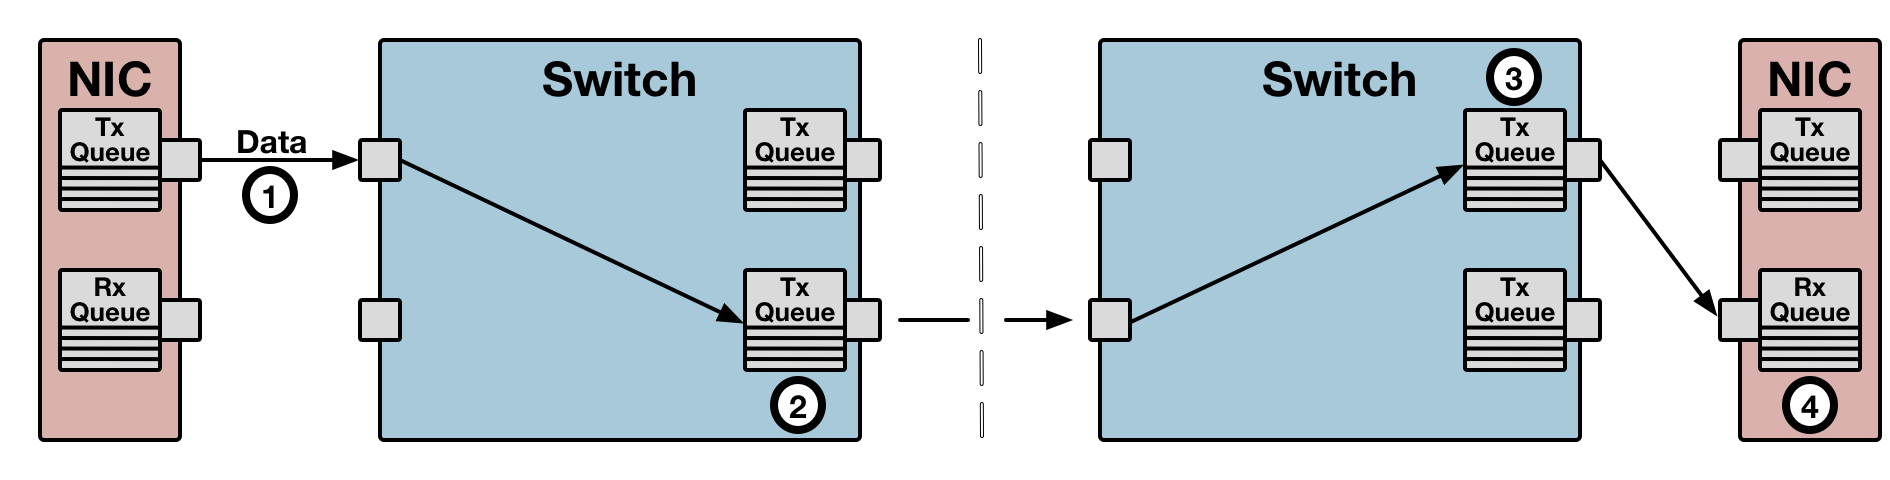
\includegraphics[width=0.9\textwidth]{figures/sculpin.png}
\caption[SCULPIN model]{SCULPIN (Simple Congestion Unbuffered Latency Packet Interconnection Network) models the main source of contention in today's networks occurring on the output port ser/des. For details on numbered steps, see text.}
\label{fig:sculpin}
\end{figure}

\subsection{SNAPPR}
\label{subsec:snappr}

Because of the coarse-grained mechanisms used in PISCES and SCULPIN, it can be difficult to model more advanced mechanisms like QoS or congestion control. 
SNAPPR (Simulator Network for Adaptive Priority Packet Routing) uses a coarse-grained cycle-based simulation that allows priority queues based on QoS or restricting injection rate for congestion control. The model is configured in much the same way as the other models.  SNAPPR is slightly more expensive than the other models, but provides by far the most flexibility and most detailed statistics.
An example file running a simple application can be found in the top-level examples folder.

\subsection{Flow}
\label{subsec:tutorial:flow}
The flow model, in simple cases, corrects the most severe problems of the packet model.
Instead of discrete chunks, messages are modeled as fluid flows moving through the network.
Congestion is treated as a fluid dynamics problem, sharing bandwidth between competing flows.
In contrast to LogP models, flow models can account fairly well for congestion.
Without congestion, a flow only requires a FLOW START and FLOW STOP event to be modeled (see tutorial on discrete event simulation in \ref{sec:tutorial:des}).
While the packet model would require many, many events to simulate a 1 MB message, the flow model might only require two.
With congestion, flow update events must be scheduled whenever congestion changes on a network link.
For limited congestion, only a few update events must occur.
The flow model also corrects the latency and multiplexing problems in the PISCES simple model, providing higher-accuracy for coarse-grained simulation.

The flow model starts to break down for large systems or under heavy congestion.
In the packet model, all congestion events are ``local'' to a given router.
The number of events is also constant in packet models regardless of congestion since we are modeling a fixed number of discrete units.
In flow models, flow update events can be ``non-local,'' propagating across the system and causing flow update events on other routers.
When congestion occurs, this ``ripple effect'' can cause the number of events to explode, overwhelming the simulator.
For large systems or heavy congestion, the flow model is actually much slower than the packet model. Support for this model has been completely removed.
